\documentclass[twocolumn=on,DIV=calc]{scrartcl}
\usepackage[portuguese]{babel}
\usepackage[colorlinks,allcolors=blue]{hyperref}
\usepackage[utf8]{inputenc}
\usepackage{microtype}
\usepackage[labelsep=period]{caption}
\usepackage{amsmath}
\usepackage{graphicx}
\newcommand{\dpar}[1]{\left(#1\right)}
\newcommand{\un}[1]{\mathrm{#1}}

\DeclareMathOperator{\sen}{sen}
\DeclareMathOperator{\pr}{pr}

\title{Física Geral I: Lista de exercícios 4}

\author{Data de entrega: 13 de junho de 2018}

\date{}

\begin{document}
\maketitle

\paragraph{Instruções}

\begin{itemize}
\item Fazer a questão correspondente ao último algarismo do seu RA. Se
  esse for $0$, faça a questão 10.
\item Além da questão anterior, faça uma outra questão de sua escolha.
\end{itemize}

\paragraph{Questões}


\begin{enumerate}
\item Uma força horizontal $\vec F$ é aplicada sobre um bloco $A$ de
  $20\,\un{kg}$ que pode deslizar sobre uma mesa sem atrito. O bloco
  $A$ está em contato com um bloco menor $B$, cuja massa é de
  $2\,\un{kg}$ (ver figura~\ref{fig:6}). Os coeficientes de atrito
  estáticos entre $A$ e $B$ são $\mu_s=0.8$ e $\mu_c=0.6$
  respectivamente. Determine o menor valor de $|\vec F|$ para que o
  bloco $B$ não caia.

  \textit{Dica:} As componentes horizontais das acelerações de ambos
  os blocos vão ser iguais.
  \begin{figure}[ht]
    \centering
    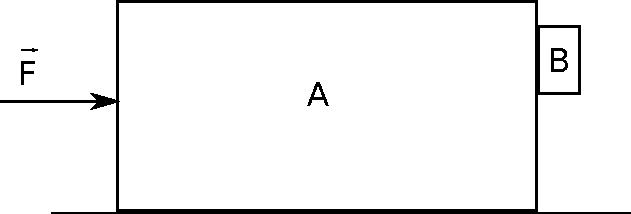
\includegraphics[width=0.4\textwidth,keepaspectratio]{lista4-questao6.pdf}
    \caption{}
    \label{fig:6}
  \end{figure}
\item Usando os dados da questão anterior, determine as componentes
  horizontal e vertical da aceleração do bloco $B$ se (i)
  $|\vec F|=300\,\un{N}$, (ii) $|\vec F|=100\,\un{N}$.
\item Uma barra de $12\,\un{kg}$ está em repouso na configuração
  mostrada na figura~\ref{fig:7}. Um dos extremos da barra está
  apoiada em uma parede e o outro está segurado por uma corda. Um
  dinamômetro foi colocado na corda para medir o valor da tensão, o
  qual marca $98\,\un{N}$. (i) Se o coeficiente de atrito estático
  entre a barra e a parede é $\mu_s=0.9$, determine a força de atrito
  sobre a barra. (ii) Determine qual é o menor valor de $\mu_s$ para
  que a barra fique em repouso.
  \begin{figure}[ht]
    \centering
    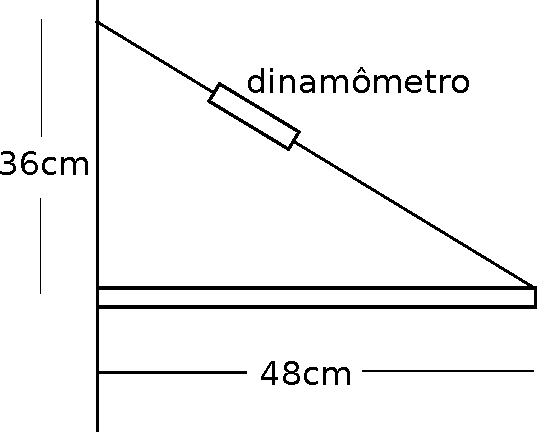
\includegraphics[width=0.35\textwidth,keepaspectratio]{lista4-questao7.pdf}
    \caption{}
    \label{fig:7}
  \end{figure}
\item A figura~\ref{fig:2} ilustra dois blocos inicialmente em repouso
  sobre uma mesa. As massas dos blocos $A$ e $B$ são $2\,\un{kg}$ e
  $5\,\un{kg}$ respectivamente. Os coeficientes de atrito estático e
  cinético entre o bloco $B$ e a mesa são $\mu_s=0{,}2$ e
  $\mu_c=0{,}1$ respectivamente. Se não há atrito entre os blocos,
  determine a aceleração dos blocos, caso eles se movam.
  \begin{figure}[ht]
    \centering
    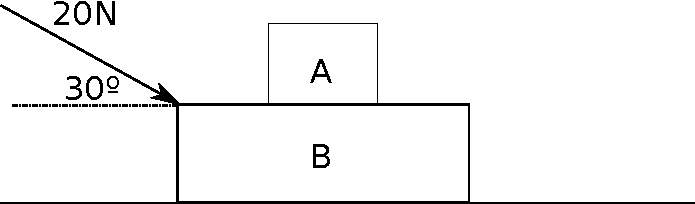
\includegraphics[width=0.45\textwidth,keepaspectratio]{lista4-questao2.pdf}
    \caption{}
    \label{fig:2}
  \end{figure}
\item A figura~\ref{fig:9} mostra dois blocos unidos por uma corda que
  passa por uma polia. Todas as superfícies são livres de atrito e as
  massas dos blocos $A$ e $B$ são $20\,\un{kg}$ e $15\,\un{kg}$
  respectivamente. (i) Se $\sen\theta=3/4$, determine os módulos e as
  direções das acelerações dos blocos. (ii) Determine o valor do
  ângulo $\theta$ para que os blocos se movam com velocidade
  constante.
  \begin{figure}[ht]
    \centering
    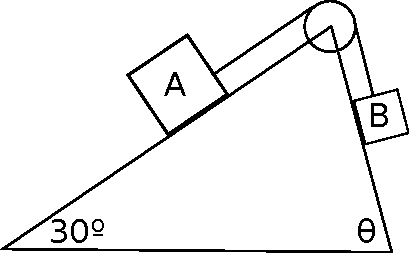
\includegraphics[width=0.3\textwidth,keepaspectratio]{lista4-questao9.pdf}
    \caption{}
    \label{fig:9}
  \end{figure}
\item Na figura~\ref{fig:4} as massas dos blocos $A$ e $B$ são
  $2\,\un{kg}$ e $5\,\un{kg}$ respectivamente. (i) Determine a
  aceleração de cada um dos blocos. (ii) Determine a tensão na corda
  que une os blocos.
  \begin{figure}[ht]
    \centering
    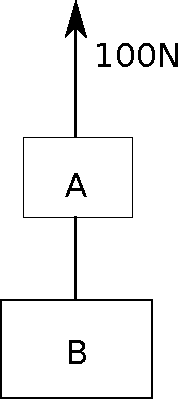
\includegraphics[width=0.12\textwidth,keepaspectratio]{lista4-questao4.pdf}
    \caption{}
    \label{fig:4}
  \end{figure}
\item A figura~\ref{fig:8} mostra dois blocos conectados por uma corda
  que passa por uma polia. As massas dos blocos $A$ e $B$ são
  $5\,\un{kg}$ e $10\,\un{kg}$ respectivamente. Se coeficiente de
  atrito cinético é $\mu_c=0.5$ entre todas as superfícies, determine
  o módulo da força $\vec F$ para que os blocos se movam com
  velocidade constante.
  \begin{figure}[ht]
    \centering
    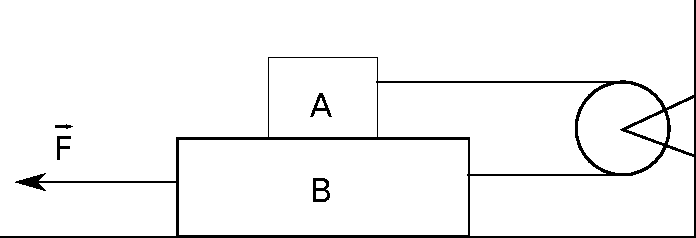
\includegraphics[width=0.4\textwidth,keepaspectratio]{lista4-questao8.pdf}
    \caption{}
    \label{fig:8}
  \end{figure}
\item Na figura~\ref{fig:5} as massas dos blocos $A$ e $B$ são
  $10\,\un{kg}$ e $5\,\un{kg}$ respectivamente. Não existe atrito
  entre o bloco $A$ e as paredes e nem com o bloco $B$ (i) Se existe
  atrito entre o bloco $B$ e o chão, determine a força de atrito sobre
  o bloco $B$ para que ele fique em repouso. (ii) Se não existe atrito
  entre o bloco $B$ e o chão, determine a aceleração do bloco $B$.

  \textit{Dica:} No item (ii) use a seguinte relação entre as
  acelerações dos blocos $A$ e $B$: $a_A=a_B\tan 60º$.
  \begin{figure}[ht]
    \centering
    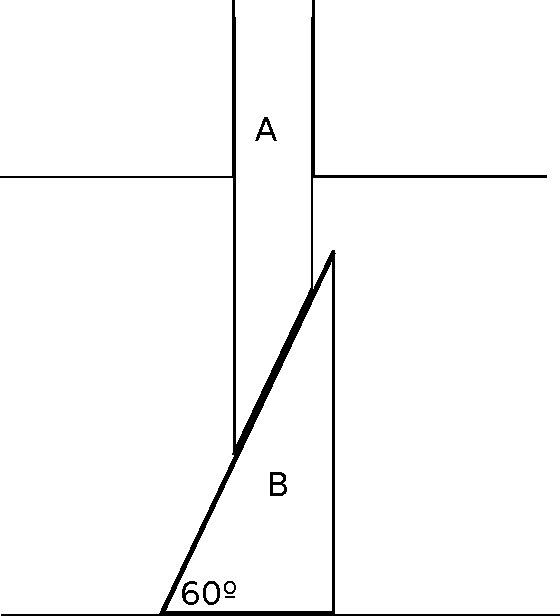
\includegraphics[width=0.3\textwidth,keepaspectratio]{lista4-questao5.pdf}
    \caption{}
    \label{fig:5}
  \end{figure}
\item Na figura~\ref{fig:3} as massas dos blocos $A$ e $B$ são
  $50\,\un{kg}$ e $100\,\un{kg}$ respectivamente. (i) Qual deve ser o
  coeficiente de atrito estático mínimo entre o bloco $B$ e o chão
  para que o bloco $A$ esteja em repouso? (ii) Se não há atrito entre
  o bloco $B$ e o chão, determine o módulo e a direção das acelerações
  dos blocos.
  \begin{figure}[ht]
    \centering
    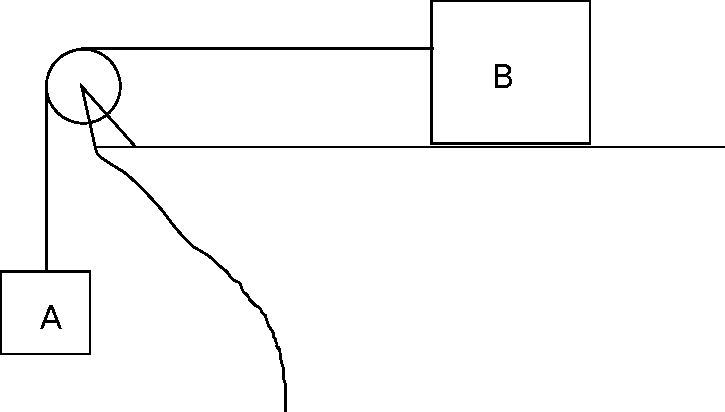
\includegraphics[width=0.4\textwidth,keepaspectratio]{lista4-questao3.pdf}
    \caption{}
    \label{fig:3}
  \end{figure}
\item Um bloco de $5\,\un{kg}$ se encontra sobre uma mesa como
  mostrado na figura~\ref{fig:1}. (i)~Determine o módulo e a direção
  da força normal sobre o bloco. (ii) Se as superfícies do bloco e da
  mesa são rugosas, determine o módulo e a direção da força de atrito
  sobre o bloco para que ele se mova com velocidade constante. (iii)
  Se todas as superfícies são lisas, determine o módulo e a direção da
  aceleração do bloco.
  \begin{figure}[ht]
    \centering
    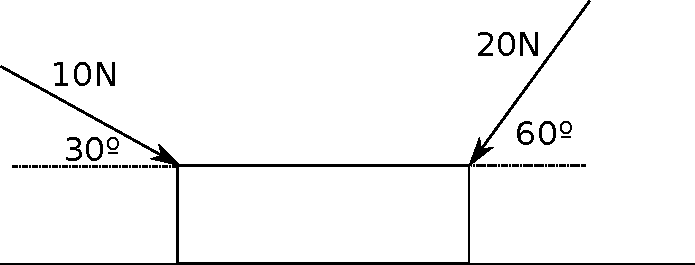
\includegraphics[width=0.45\textwidth,keepaspectratio]{lista4-questao1.pdf}
    \caption{}
    \label{fig:1}
  \end{figure}
\end{enumerate}
\end{document}